\chapter{Tecnologías Utilizadas}
\label{cap:tecnologiasUtilizadas}

En este capítulo se presentan las principales tecnologías, modelos y herramientas empleados en el desarrollo del sistema, explicando su funcionamiento general y el papel que desempeñan dentro del pipeline. El objetivo no es describir la implementación concreta del proyecto, sino introducir los fundamentos necesarios.

\section{Detección de objetos con YOLO}
\label{sec:yolo-tecnologias}

La detección de objetos es una de las tareas principales dentro de la visión por computador. Su objetivo es localizar e identificar las instancias de una o varias clases presentes en una imagen, normalmente mediante cajas \textit{bounding box} asociadas a una etiqueta y a una puntuación de confianza. En esta sección se describe cómo YOLO afronta este problema.

\subsection{Modelo de detección YOLO}

Uno de los enfoques más utilizados para detección en tiempo real es YOLO \citep{RedmonYOLO2016}. Esta red neuronal convolucional plantea la detección como un problema de regresión directa sobre la imagen completa, prediciendo cajas y clases en una sola pasada. Esta filosofía de detector de una etapa resulta especialmente adecuada para vídeo, donde no basta con obtener buena precisión en imágenes aisladas, sino que también es importante mantener una velocidad de inferencia suficiente para procesar secuencias largas. Las implementaciones modernas de Ultralytics \citep{UltralyticsYOLO2023} \footnote{Ultralytics es una empresa y comunidad de desarrollo de software especializada en herramientas de visión por computador, conocida principalmente por mantener implementaciones modernas de YOLO y facilitar su entrenamiento, evaluación y despliegue.} han popularizado su uso práctico mediante modelos preentrenados, herramientas de entrenamiento y despliegue, y soporte para fine-tuning sobre datasets propios.


En la formulación original de YOLO, la imagen se divide en una cuadrícula de $S \times S$ celdas. Cada celda es responsable de predecir los objetos cuyo centro cae dentro de ella. Para cada celda, la red estima una o varias cajas delimitadoras junto con una confianza de objeto y una distribución de probabilidad sobre las clases. De forma simplificada, cada predicción puede representarse como:

\[
(x, y, w, h, C)
\]

donde $x$ e $y$ indican la posición del centro de la caja, $w$ y $h$ representan su anchura y altura, y $C$ expresa la confianza asociada a la existencia de un objeto y a la calidad de la localización. Además, la red predice las probabilidades de clase. La puntuación final de una detección puede entenderse como la combinación entre la confianza de objeto y la probabilidad de clase:

\[
score = P(\text{objeto}) \cdot P(\text{clase} \mid \text{objeto})
\]

El flujo de este modelo de detección se muestra en la \hyperref[fig:yolo-grid]{Figura~\ref*{fig:yolo-grid}}. La red comparte un mismo \textit{backbone} para extraer características visuales de la imagen y, a partir de ellas, produce simultáneamente la regresión de cajas, la confianza y la clasificación. Aunque las versiones modernas de YOLO utilizadas por implementaciones como Ultralytics han evolucionado respecto al modelo original, incorporando cabezas de detección multiescala y mejores funciones de pérdida, la idea central sigue siendo la misma: obtener cajas y clases directamente en una única pasada de la red.

\begin{figure}[H]
    \centering
    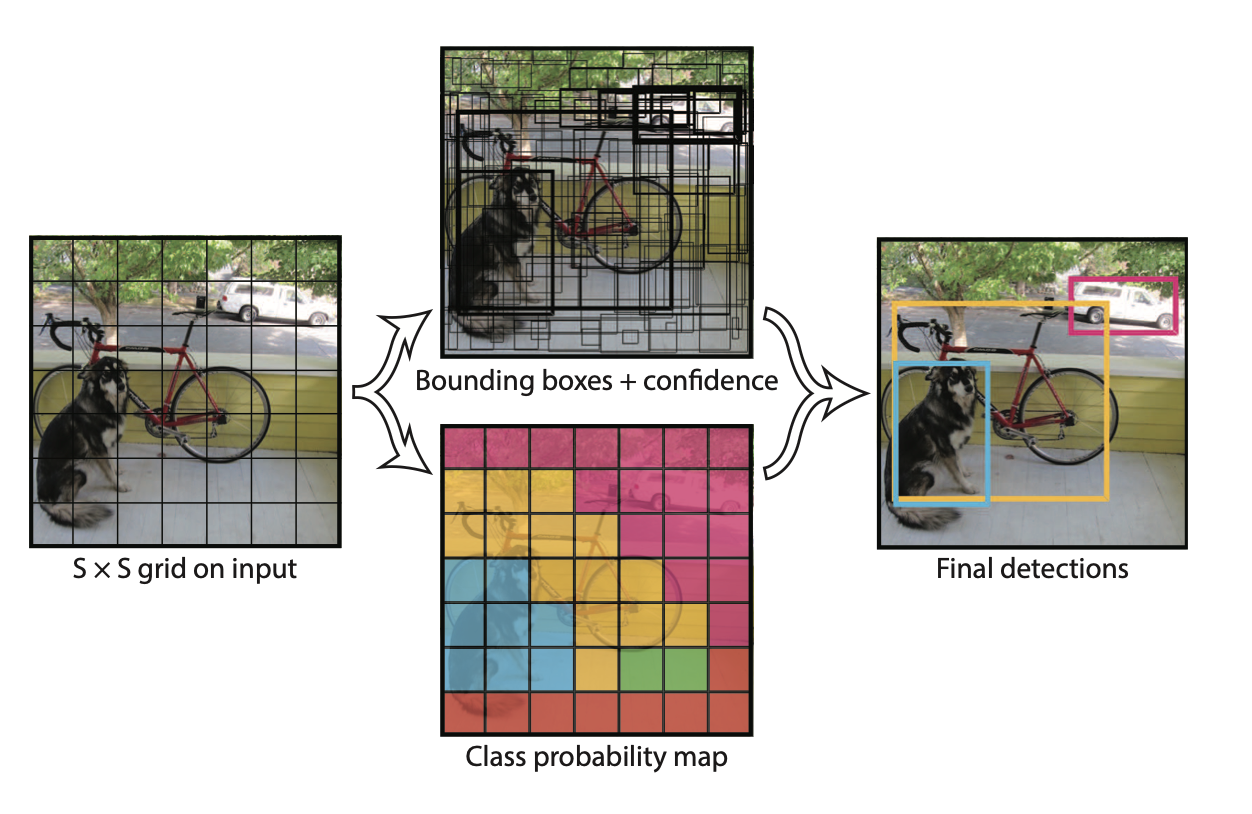
\includegraphics[width=0.9\textwidth]{Imagenes/Propias/YOLO2.png}
    \caption[Esquema conceptual de YOLO como detector de una etapa]{Esquema conceptual de YOLO como detector de una etapa: división espacial, regresión de cajas y clasificación. Fuente: reproducido de \citep{RedmonYOLO2016}.}
    \label{fig:yolo-grid}
\end{figure}

Durante el entrenamiento, la función de pérdida combina varios objetivos. Por un lado, penaliza el error de localización entre la caja predicha y la caja real. Por otro lado, penaliza los errores de confianza, diferenciando entre regiones que contienen objetos y regiones de fondo. Finalmente, incorpora el error de clasificación. Esto obliga al modelo a aprender simultáneamente tres tareas: localizar el objeto, decidir si realmente existe y asignarle una clase correcta.

\subsection{Post-procesado mediante Non-Maximum Suppression}
Tras la inferencia, es habitual que el detector produzca varias cajas muy próximas para un mismo objeto. Para eliminar estas detecciones redundantes se aplica \textit{Non-Maximum Suppression} (NMS). Este algoritmo ordena las cajas por puntuación, conserva la de mayor confianza y elimina aquellas cajas de la misma clase cuyo solape con ella supere un determinado umbral. El solape se mide mediante la intersección sobre la unión, o IoU:

\[
IoU(A,B)=\frac{\operatorname{area}(A \cap B)}{\operatorname{area}(A \cup B)}
\]

Si dos cajas tienen un IoU superior al umbral $\lambda_{nms}$, se considera que ambas representan el mismo objeto y se conserva únicamente la de mayor confianza. La \hyperref[fig:yolo-nms]{Figura~\ref*{fig:yolo-nms}} ilustra este proceso, en el que múltiples predicciones cercanas se reducen a una única caja final. Esto también puede observarse en el segundo paso de la \hyperref[fig:yolo-grid]{Figura~\ref*{fig:yolo-grid}}.

\begin{figure}[H]
    \centering
    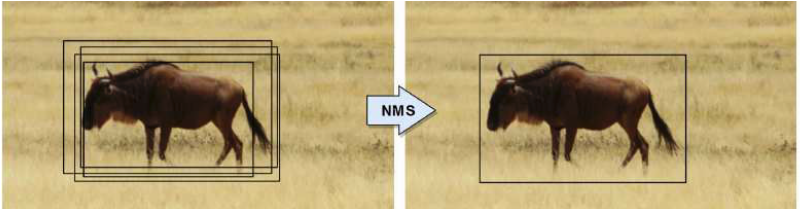
\includegraphics[width=0.9\textwidth]{Imagenes/Propias/YOLO1.png}
    \caption[Postproceso mediante Non-Maximum Suppression]{Postproceso mediante Non-Maximum Suppression para eliminar cajas redundantes.
    Fuente: reproducido de \citep{BesadaAnalisisSenal2025}}
    \label{fig:yolo-nms}
\end{figure}


\subsection{Métricas de evaluación en detección de objetos}
\label{subsec:metricas-deteccion-objetos}

Para evaluar un detector de objetos no basta con comprobar si predice la clase correcta, sino que también es necesario analizar la calidad de la localización espacial. Para ello se utiliza habitualmente la IoU. Una detección se considera correcta si su IoU supera un determinado umbral y la clase predicha coincide con la clase real.

A partir de esta correspondencia entre predicciones y anotaciones reales se calculan métricas como la precisión y el recall. La precisión mide qué proporción de las detecciones realizadas por el modelo son correctas, mientras que el recall mide qué proporción de los objetos reales han sido detectados. Estas métricas se definen como:

\[
\text{Precisión} = \frac{TP}{TP + FP}
\]

\[
\text{Recall} = \frac{TP}{TP + FN}
\]

donde $TP$ representa el número de verdaderos positivos, $FP$ el número de falsos positivos y $FN$ el número de falsos negativos. En el contexto de la detección de objetos, un verdadero positivo corresponde a una predicción cuya clase es correcta y cuya IoU con la caja real supera el umbral establecido. Un falso positivo es una detección incorrecta o duplicada, mientras que un falso negativo corresponde a un objeto real que no ha sido detectado.

El valor F1 combina ambas métricas mediante su media armónica:

\[
F1 = 2 \cdot \frac{\text{Precisión} \cdot \text{Recall}}{\text{Precisión} + \text{Recall}}
\]

Esta métrica resulta útil cuando se desea valorar conjuntamente falsos positivos, asociados a la precisión, y falsos negativos, asociados al recall.

En detección de objetos también es habitual emplear la métrica mAP (\textit{mean Average Precision}). El mAP@50 considera correcta una detección cuando alcanza un IoU mínimo de 0.50, mientras que el mAP@50-95 calcula el rendimiento medio usando varios umbrales de IoU entre 0.50 y 0.95.


\subsection{Papel de YOLO dentro del pipeline}
En este proyecto, YOLO se utiliza como detector inicial del pipeline para localizar jugadores, árbitros, porteros y balón en cada fotograma. Sus salidas sirven como entrada para las etapas posteriores de seguimiento y análisis temporal.

En esta sección se ha introducido YOLO desde un punto de vista conceptual. Su aplicación concreta dentro del sistema se desarrolla posteriormente en la \hyperref[sec:deteccion-elementos-juego]{Sección~\ref*{sec:deteccion-elementos-juego}, Detección de elementos del juego}.

% \section{Analisis de color mediante CIE LAB y KMeans}
\subsection{Espacios de color y color dominante}
El análisis de color es una técnica utilizada en visión por computador para describir, comparar y agrupar regiones de una imagen a partir de su apariencia cromática. Este tipo de información puede resultar útil cuando se desea distinguir elementos visualmente similares en forma o tamaño, pero diferenciados por su color dominante.

Desde el punto de vista clásico, una estrategia sencilla y eficiente consiste en extraer el color dominante de una región de interés obtenida a partir de una detección. El uso directo del espacio RGB puede ser problemático, porque mezcla información cromática y luminancia, de modo que cambios de iluminación, sombras o balance de blancos alteran de forma significativa las distancias entre colores. Por ello, resulta habitual transformar la imagen a espacios más adecuados para comparación perceptual, como CIE L*a*b*, donde el canal L* representa la luminosidad y los canales a* y b* codifican los ejes cromáticos \citep{cie1976lab}. Esta separación permite que las diferencias de color sean más estables que en RGB cuando varían las condiciones de captura.

Sobre este espacio de color puede aplicarse \textit{k-means}, un algoritmo de agrupamiento no supervisado que divide un conjunto de muestras en $K$ grupos minimizando la suma de distancias cuadráticas a sus centroides \citep{macqueen1967kmeans,lloyd1982least}:

\[
\min_{\mu_1,\dots,\mu_K} \sum_{i=1}^{n} \min_{k \in \{1,\dots,K\}} \|x_i - \mu_k\|_2^2
\]

Aplicado al análisis de imagen, cada muestra puede corresponder a un píxel o a una representación cromática extraída de una región. El resultado del agrupamiento permite identificar colores dominantes y separar componentes visuales con apariencia distinta. Esta técnica tiene la ventaja de no requerir entrenamiento supervisado y de poder adaptarse a cada imagen o secuencia de entrada. Sin embargo, su rendimiento puede verse afectado cuando los colores son muy parecidos, cuando la región analizada contiene demasiado fondo o cuando existen cambios fuertes de iluminación.

\subsection{Papel del análisis de color dentro del pipeline}
En el contexto de este proyecto, el análisis de color se utiliza para apoyar la identificación automática de equipos a partir del color de camiseta de los jugadores. Una vez detectado un jugador, el recorte asociado a su \textit{bounding box} contiene información visual que puede emplearse para estimar el color dominante de la camiseta y compararlo con el de otros jugadores.

Esta idea puede aplicarse en dos niveles. En primer lugar, dentro del recorte de cada jugador, para separar la camiseta de otros píxeles pertenecientes al fondo, al césped, a la piel o al pantalón. En segundo lugar, sobre los colores dominantes estimados para varios jugadores, para agruparlos en los dos equipos principales. De esta forma, la información cromática se convierte en una señal adicional que puede utilizarse en etapas posteriores del sistema, especialmente en el tracking multiobjeto y en la generación de una representación estructurada del partido.

Frente a un clasificador supervisado de camisetas, esta solución tiene la ventaja de no requerir un conjunto de entrenamiento específico para cada partido y de poder adaptarse al inicio de cada vídeo. Su principal limitación aparece cuando ambos equipos usan colores parecidos, cuando el recorte incluye demasiado fondo o cuando la cámara introduce cambios fuertes de exposición.
\section{Calibración geométrica mediante homogarfía}
\label{sec:homografia-tecnologias}
En muchos problemas de visión por computador, las coordenadas observadas en una imagen no representan directamente la posición real de los objetos en la escena. La perspectiva, el zoom, la posición de la cámara y los movimientos de la misma pueden hacer que dos puntos separados por la misma distancia física aparezcan a distancias muy distintas en píxeles. Por este motivo, cuando se desea razonar sobre posiciones reales, resulta necesario calibrar la cámara y transformar puntos desde el plano de la imagen hacia un plano de referencia.

\subsection{Homografía entre planos}

Cuando la superficie observada puede aproximarse como un plano, la relación entre los puntos de la imagen y los puntos de dicho plano puede modelarse mediante una homografía. Una homografía es una transformación proyectiva \footnote{Una transformación proyectiva es una operación geométrica que mapea puntos de un plano (o espacio) a otro, preservando las líneas rectas pero no necesariamente el paralelismo, ángulos o distancias} entre dos planos, representada mediante una matriz $H \in \mathbb{R}^{3 \times 3}$. En este contexto, permite relacionar coordenadas en píxeles de la imagen broadcast con coordenadas sobre una representación 2D del terreno de juego.

Para expresar esta transformación se utilizan coordenadas homogéneas. Este tipo de representación consiste en añadir a un punto bidimensional como $(u,v)$, una tercera componente y se escribe como $(u,v,1)$. Esta representación permite describir transformaciones de perspectiva mediante una multiplicación matricial. Así, un punto de imagen $(u,v)$ y su correspondiente punto del plano de referencia $(x,y)$ se relacionan mediante:

\[
\begin{bmatrix}
x \\
y \\
1
\end{bmatrix}
\sim
H
\begin{bmatrix}
u \\
v \\
1
\end{bmatrix}
\]

Tras aplicar la matriz, las coordenadas resultantes se normalizan dividiendo por la tercera componente para volver a obtener coordenadas bidimensionales.

La \hyperref[fig:exp-homografia]{Figura~\ref*{fig:exp-homografia}} muestra una interpretación geométrica de esta idea, en la que los puntos de un plano se proyectan sobre otro plano, estableciendo una correspondencia entre ambas superficies.

\begin{figure}[H]
    \centering
    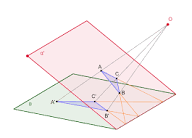
\includegraphics[width=0.3\textwidth]{Imagenes/Propias/exp_homografia.png}
    \caption[Esquema de homografía entre planos]{
Esquema geométrico de una homografía entre dos planos proyectivos. Los puntos del plano original se proyectan desde un centro de proyección sobre un segundo plano, estableciendo una correspondencia entre ambas superficies. Fuente: reproducida de \citep{DibujoSecundariaTransformaciones}.
}
    \label{fig:exp-homografia}
\end{figure}

Esta transformación no conserva necesariamente distancias, ángulos ni áreas, pero sí permite transformar puntos entre dos planos cuando existen suficientes correspondencias geométricas. Estas correspondencias pueden obtenerse a partir de elementos conocidos de la escena. Si se identifican suficientes referencias, es posible estimar la homogradia que alinea la imagen con una representación métrica del plano observado.

\subsection{Estimación de homografía mediante PnLCalib}
PnLCalib \citep{GutierrezPnLCalib2024} es un método de calibración de cámaras en vídeo deportivo diseñado para obetener una transformación geométrica que permita proyectar la imagen broadcast sobre un modelo geométrico del campo de fútbol. A diferencia de otros enfoques que dependen únicamente de puntos característicos o de una búsqueda sobre posibles poses de cámara, PnLCalib combina información de puntos y líneas del terreno de juego para obtener una estimación más robusta.

El método parte de una idea sencilla: el campo de fútbol tiene una geometría conocida. Líneas de banda, áreas, círculo central, puntos de penalti e intersecciones entre marcas del terreno pueden utilizarse como referencias para estimar la relación entre la imagen y el modelo del campo. Para ello, PnLCalib emplea redes encoder-decoder que predicen mapas de calor de \textit{keypoints} y extremos de líneas visibles en el frame. A partir de estas predicciones se extraen correspondencias entre la imagen y el modelo geométrico del campo.

El proceso general de PnLCalib se resume en la \hyperref[fig:pnlcalib-pipeline]{Figura~\ref*{fig:pnlcalib-pipeline}} y se divide en dos etapas principales: la generación de datos de entrenamiento y la fase de inferencia.

En la primera etapa, el método parte de las anotaciones de SoccerNet y de la geometría conocida del campo de fútbol para construir las referencias que aprenderán las redes. El resultado de esta etapa no es un nuevo conjunto de imágenes, sino un conjunto de pares de entrenamiento en los que cada frame queda asociado a 57 mapas de calor que indican la posición esperada de 57 puntos característicos del terreno de juego y a 23 mapas de calor de las líneas del campo.

Durante la fase de inferencia, PnLCalib recibe un frame de entrada y utiliza dos redes encoder-decoder. La primera red predice $57+1$ mapas de calor: un canal para cada \textit{keypoint} predefinido y un canal adicional de fondo. Cada mapa de calor indica la probabilidad de que el punto correspondiente se encuentre en cada posición de la imagen, por lo que la localización final del punto se obtiene seleccionando las zonas de mayor activación. La segunda red predice $23+1$ mapas de calor asociados a las líneas del campo: un canal por cada línea considerada y un canal adicional de borde. En este caso, cada canal contiene dos activaciones principales, correspondientes a los extremos visibles de la línea.

A partir de los máximos de estos mapas de calor se extraen las posiciones en la imagen de los puntos característicos y de los extremos de las líneas en la imagen. Además, las líneas detectadas pueden utilizarse para recuperar puntos no observados directamente mediante intersecciones entre líneas, aumentando así el número de referencias disponibles. Además las posiciones en el modelo del campo de todas esas referencias son conocidas, por tanto, con estas correspondencias entre la imagen y el modelo geométrico del campo se calcula una calibración inicial mediante métodos geométricos.

Finalmente, PnLCalib incorpora un módulo de refinamiento PnL, de \textit{Points and Lines}, que ajusta la calibración inicial utilizando conjuntamente la información de puntos y líneas. Este refinamiento se plantea como un problema de optimización no lineal orientado a reducir el error de reproyección, es decir, la diferencia entre las referencias observadas en la imagen y las referencias proyectadas desde el modelo geométrico del campo.

\begin{figure}[H]
    \centering
    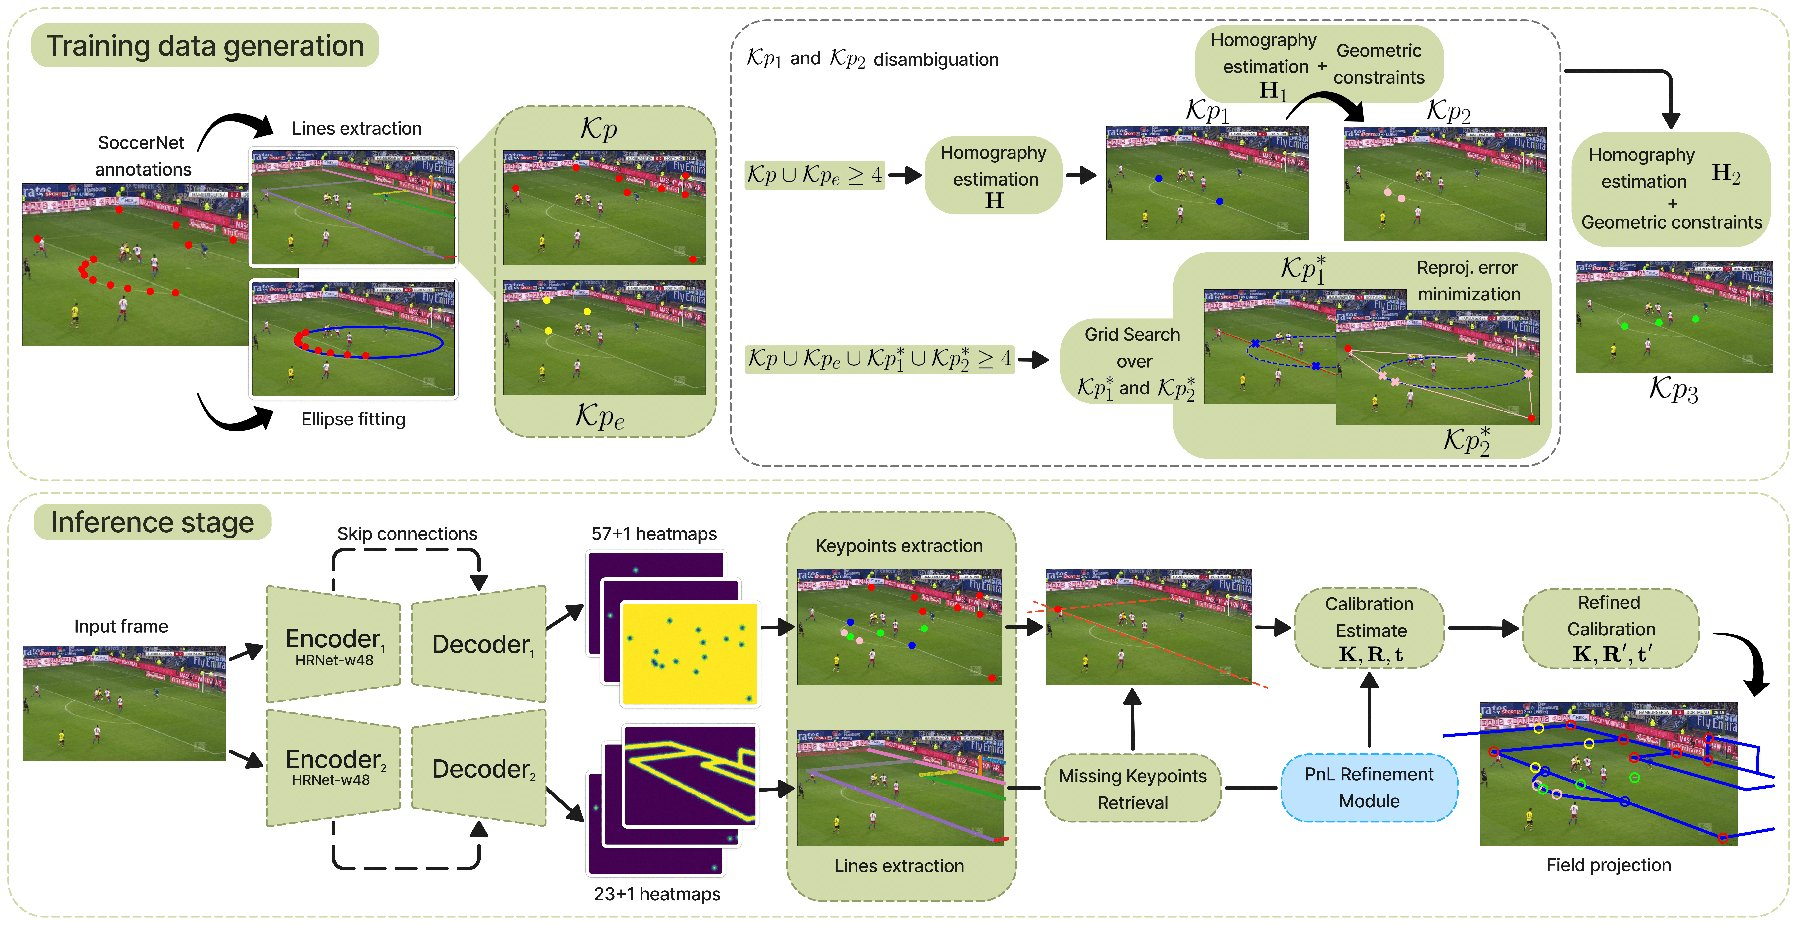
\includegraphics[width=0.9\textwidth]{Imagenes/Propias/pipeline.jpg}
    \caption[Pipeline de PnLCalib]{
    Pipeline de PnLCalib para estimar la calibración del campo mediante \textit{keypoints}, líneas y refinamiento geométrico. Fuente: reproducida de \citep{GutierrezPnLCalib2024}.
    }
    \label{fig:pnlcalib-pipeline}
\end{figure}

La \hyperref[fig:field-reconstruction]{Figura~\ref*{fig:field-reconstruction}} muestra un ejemplo visual de este proceso. Las líneas proyectadas representan la estructura geométrica estimada del campo sobre la imagen original, mientras que los puntos coloreados indican referencias detectadas o utilizadas durante el ajuste. Este tipo de visualización permite comprobar de forma intuitiva si la calibración obtenida es coherente con la escena observada.

\begin{figure}[H]
    \centering
    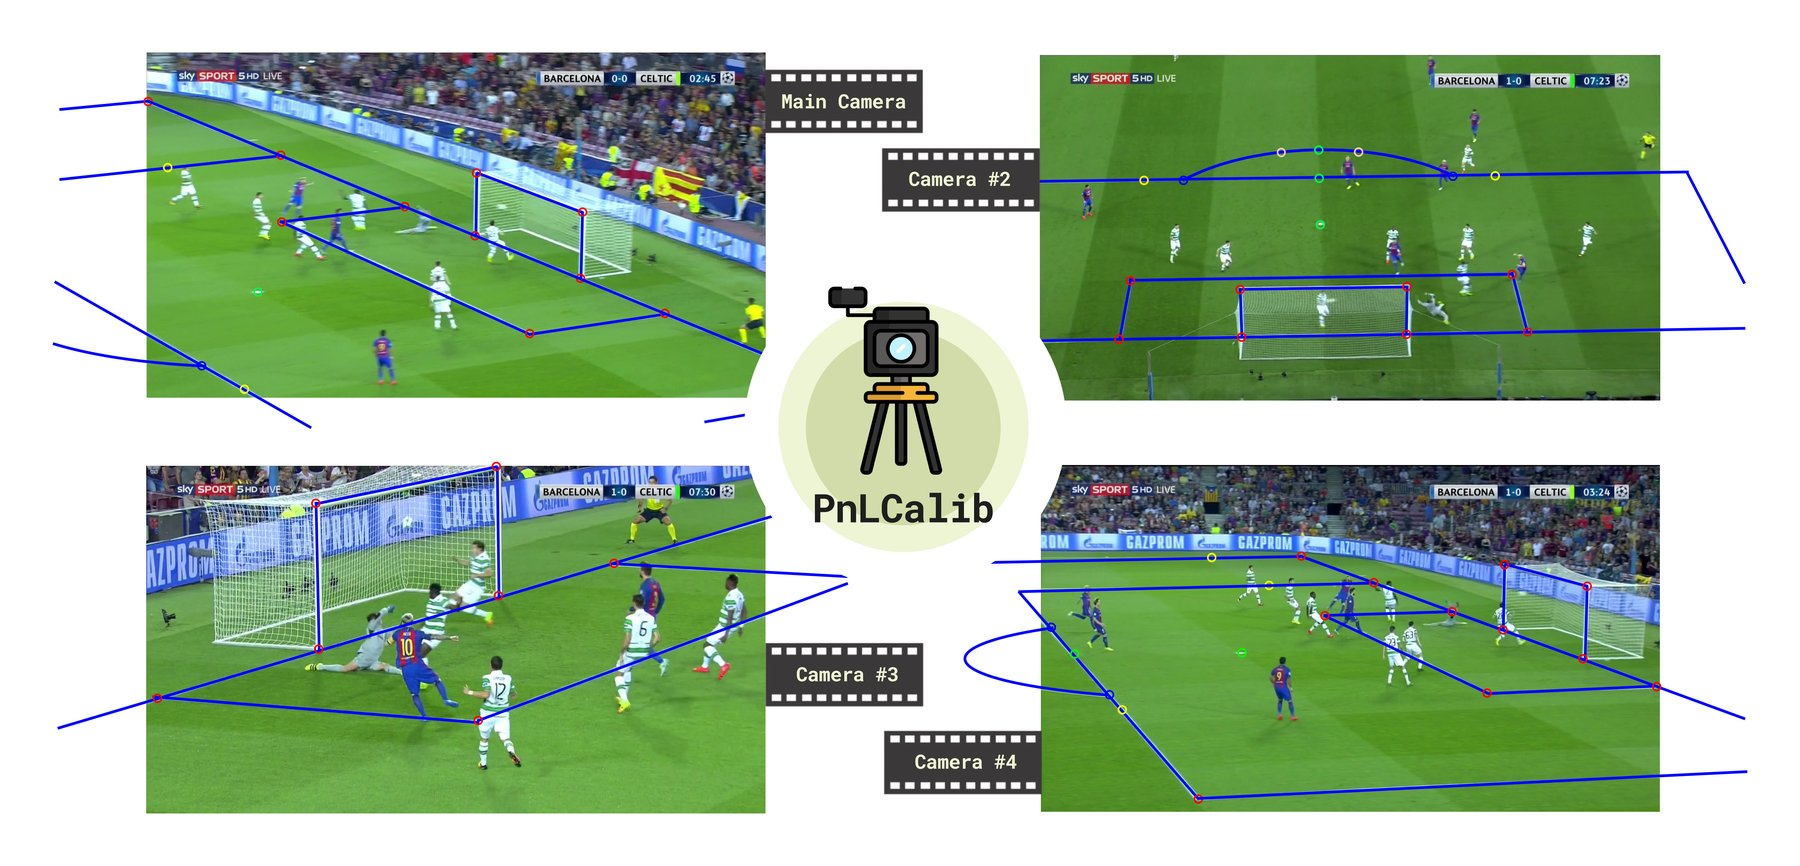
\includegraphics[width=0.95\textwidth]{Imagenes/Propias/field_reconstruction.jpg}
    \caption[Reconstrucción geométrica sobre imágenes broadcast]{
    Reconstrucción geométrica sobre imágenes broadcast mediante líneas y puntos de referencia. Fuente: reproducida de \citep{PnLCalibRepo2024}.
    }
    \label{fig:field-reconstruction}
\end{figure}

\subsection{Papel de la homografía dentro del pipeline}
En el contexto de este proyecto, la homografía permite transformar las detecciones obtenidas en la imagen broadcast hacia una representación 2D del terreno de juego. De esta forma, las detecciones obtenidas en píxeles pueden expresarse en un sistema de coordenadas más próximo al espacio físico real del partido.

Una vez estimada la homografía, cada detección puede proyectarse al campo a partir de un punto representativo. En el caso de los jugadores, se utiliza habitualmente el punto inferior central de la \textit{bounding box}, ya que aproxima la posición de contacto del jugador con el plano del suelo.

La principal ventaja de trabajar en coordenadas del campo es que las distancias pasan a tener una interpretación física. Esto resulta útil para etapas posteriores del pipeline, como el tracking multiobjeto, la clasificación posicional o el análisis de eventos. Por ejemplo, una identidad perdida puede recuperarse si reaparece en una posición compatible sobre el terreno de juego.

No obstante, la calibración también introduce riesgos. Si la homografía estimada es incorrecta, todas las posiciones proyectadas quedarán desplazadas de forma sistemática. En vídeo broadcast, este problema puede aparecer cuando la cámara cambia bruscamente, cuando se observa una zona reducida del campo o cuando las líneas visibles son insuficientes. Por este motivo, la homografía debe tratarse como una señal valiosa, pero no infalible, y conviene que el pipeline pueda continuar aunque algunos frames no dispongan de una proyección fiable.

La integración concreta de la calibración en el sistema desarrollado, incluyendo las estrategias de robustez y los criterios prácticos de aceptación de homografías, se describe posteriormente en la 
\hyperref[sec:calibracion-campo-proyeccion-metricas]{Sección~\ref*{sec:calibracion-campo-proyeccion-metricas}}

\section{Tracking multiobjeto}
\label{sec:tracking-tecnologias}

El tracking multiobjeto consiste en mantener la identidad de múltiples objetos a lo largo de una secuencia de vídeo. A diferencia de la detección de objetos, que produce resultados independientes en cada frame, el tracking introduce una asociación temporal entre detecciones consecutivas. Su objetivo es asignar un identificador persistente a cada objeto, de forma que pueda reconstruirse su trayectoria a lo largo del tiempo.

Este problema suele abordarse combinando detección, predicción de movimiento y asociación de detecciones. En cada frame, el detector proporciona un conjunto de cajas candidatas. A continuación, el tracker compara estas detecciones con las trayectorias activas y decide qué detección corresponde a cada identidad previa, qué objetos han desaparecido temporalmente y qué detecciones deben iniciar nuevas trayectorias. Esta asociación puede basarse en medidas geométricas, como el solape entre cajas, la distancia entre posiciones o la coherencia del movimiento estimado.

\subsection{ByteTrack}
ByteTrack \citep{ZhangByteTrack2022} es una de las referencias recientes más relevantes en tracking multiobjeto. Su principal aportación consiste en no descartar directamente las detecciones con baja confianza, ya que algunas de ellas pueden corresponder a objetos reales parcialmente ocluidos, lejanos o difíciles de detectar. En lugar de ello, ByteTrack utiliza estas detecciones en una segunda etapa de asociación, lo que permite recuperar trayectorias que otros métodos podrían fragmentar.

El funcionamiento de ByteTrack puede entenderse como un ciclo que se repite en cada frame. En primer lugar, el detector proporciona un conjunto de cajas con sus puntuaciones de confianza. Estas detecciones se separan en dos grupos mediante umbrales: detecciones de alta confianza, que se consideran más fiables, y detecciones de baja confianza, que no son suficientes para iniciar nuevas trayectorias pero sí pueden servir para actualizar trayectorias ya existentes.

Antes de realizar la asociación, las trayectorias activas se predicen hacia el frame actual mediante un filtro de Kalman \citep{Kalman1960}. Este filtro estima la posición esperada de cada objeto a partir de su estado anterior, habitualmente representado mediante la posición y tamaño de la caja. De esta forma, el tracker no compara las nuevas detecciones con la última posición observada sin más, sino con una predicción de dónde debería encontrarse cada objeto en el frame actual.

La asociación se realiza en varias fases. En la primera fase, ByteTrack compara las trayectorias activas y perdidas recientemente con las detecciones de alta confianza. Para ello calcula una matriz de costes basada normalmente en la IoU entre cajas, de modo que una detección se asocia a una trayectoria si su solape con la predicción del track es suficientemente alto. Las asociaciones válidas actualizan el estado del track y mantienen su identidad.

Después, las trayectorias que no han podido asociarse en la primera fase se comparan con las detecciones de baja confianza. Esta segunda asociación es la característica distintiva de ByteTrack. Una detección de baja confianza no se utiliza para crear un nuevo objeto, ya que podría ser ruido o fondo, pero sí puede ser útil para mantener una trayectoria ya existente cuando el detector ha reducido temporalmente su seguridad. De este modo, un jugador parcialmente oculto o detectado con baja confianza puede seguir asociado a su identidad previa.

Además de los tracks activos, ByteTrack mantiene otros estados internos. Los tracks no confirmados corresponden normalmente a trayectorias recién creadas que todavía no han sido observadas durante suficientes frames (si no se asocian de nuevo rápidamente, se eliminan). Los tracks perdidos son identidades que no han encontrado una detección compatible en el frame actual, pero que se conservan durante un número limitado de frames por si el objeto reaparece. Si un track permanece perdido durante más tiempo del permitido por el parámetro de memoria del tracker, se marca como eliminado. Finalmente, las detecciones de alta confianza que no han sido asociadas a ningún track existente pueden iniciar nuevas trayectorias si superan un umbral mínimo de confianza.

La \hyperref[fig:bytetrack-esquema]{Figura~\ref*{fig:bytetrack-esquema}} resume este proceso. Primero se realiza la asociación con detecciones de alta confianza. Después, las trayectorias no asociadas se comparan con detecciones de baja confianza. Luego, las trayectorias no confirmadas se comparan con detecciones de alta confianza. Por último, se actualizan los estados de las trayectorias, se crean nuevos tracks cuando procede y se eliminan aquellos que han permanecido perdidos durante demasiado tiempo.

\begin{figure}[H]
    \centering
    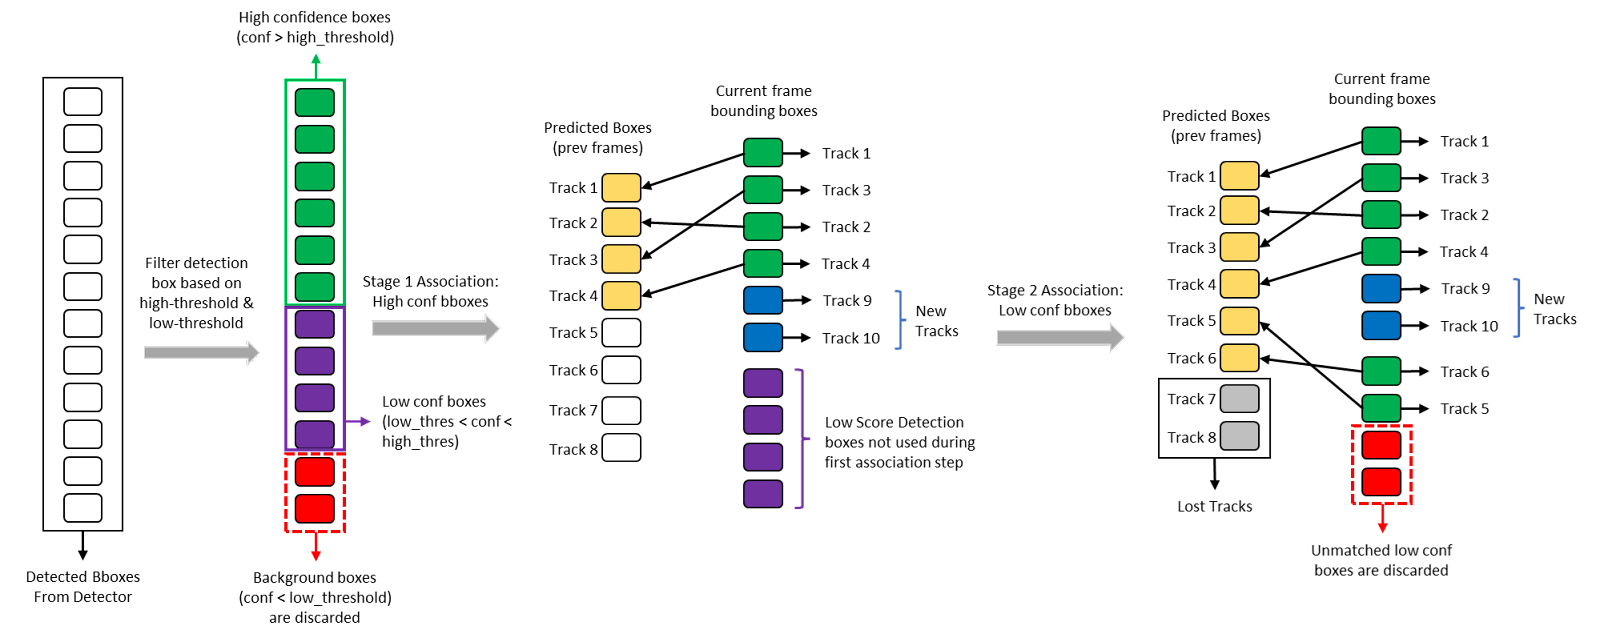
\includegraphics[width=0.9\textwidth]{Imagenes/Propias/ByteTrack.png}
    \caption[Esquema general de ByteTrack]{Esquema general de ByteTrack. El método separa las detecciones en cajas de alta y baja confianza y realiza la asociación en dos etapas, permitiendo recuperar objetos que un tracker convencional descartaría prematuramente. Fuente: reproducido de So \citep{SoByteTrack2025}.}
    \label{fig:bytetrack-esquema}
\end{figure}

Esta estrategia resulta especialmente útil en secuencias con oclusiones, movimiento rápido, cambios de escala o detecciones intermitentes. Además, ByteTrack mantiene una arquitectura relativamente simple y eficiente, ya que basa la asociación principalmente en predicción de movimiento, solape espacial y confianza de detección, sin depender necesariamente de descriptores complejos de apariencia. Esto facilita su integración en sistemas donde la latencia y la estabilidad temporal son factores importantes.

\subsection{Papel del tracking dentro del pipeline}

En este proyecto, el tracking multiobjeto permite transformar las detecciones independientes de cada frame en trayectorias persistentes de jugadores, árbitros, porteros y balón. Esta continuidad temporal es necesaria para analizar la evolución del juego y para que módulos posteriores, como la clasificación posicional o la detección de eventos puedan trabajar sobre identidades estables y analizar su evolución temporal.

El vídeo broadcast de fútbol plantea dificultades específicas para esta tarea: oclusiones frecuentes, cruces entre jugadores, similitud visual entre miembros del mismo equipo, cambios de escala, movimientos de cámara y detecciones intermitentes. Por ello, ByteTrack se utiliza como base del sistema, pero se adapta al dominio futbolístico incorporando señales adicionales y restricciones sobre las asociaciones posibles.

En nuestro caso, ByteTrack se utiliza como punto de partida, pero se realiza una profunda adaptación a nuestro caso de uso. El objetivo es aprovechar la estructura eficiente de ByteTrack, incorporando al mismo tiempo información específica del fútbol. Por tanto, el criterio de asociación no se basa únicamente en la IoU entre cajas, sino que también considera la clase detectada, el equipo estimado, la distancia entre centros de las cajas y, cuando está disponible, la posición proyectada sobre el terreno de juego. Además, se introducen restricciones duras para evitar asociaciones incompatibles y fases adicionales de asociación para recuperar correspondencias cuando el solape entre cajas no resulta suficiente.

Estas adaptaciones buscan reducir cambios de identidad, trayectorias fragmentadas y asociaciones incoherentes, problemas especialmente relevantes en un entorno como el fútbol. La implementación concreta de la capa de asociación basada en ByteTrack dentro del pipeline se describe posteriormente en la \hyperref[sec:bytetrack-layer]{Sección~\ref*{sec:bytetrack-layer}}.
\section{Modelado de conjuntos con Set Transformer}
\label{sec:setTransformer}

En esta sección se introducen los modelos Set Transformer, una arquitectura diseñada para procesar conjuntos de elementos sin imponer un orden sobre ellos. Este tipo de modelo resulta útil cuando la predicción depende tanto de las características individuales de cada elemento como de las relaciones entre todos los elementos del conjunto.

\subsection{Representación de datos como conjuntos}
En muchos problemas de aprendizaje automático, los datos de entrada no tienen una estructura secuencial natural, sino que aparecen como un conjunto de elementos. En estos casos, el orden en el que se presentan los elementos al modelo no debería modificar la salida. Por ejemplo, si un modelo recibe un conjunto de vectores que describen distintos objetos de una escena, permutar el orden de esos vectores no debería cambiar la interpretación global de la escena. 

Los modelos clásicos basados en redes densas no incorporan esta propiedad de forma directa, ya que suelen asumir que cada posición de la entrada tiene un significado fijo. Una alternativa consiste en procesar cada elemento de forma independiente y después aplicar una operación agregadora, como suma, media o máximo. Sin embargo, este tipo de aproximaciones puede ser limitado cuando la predicción depende de las relaciones entre los elementos del conjunto. Para capturar estas dependencias, las arquitecturas Set Transformer \citep{lee2019settransformer} proponen utilizar mecanismos de atención adaptados al procesamiento de conjuntos.

\subsection{Atención multi-cabeza en conjuntos}
Set Transformer se basa en el mecanismo de atención multi-cabeza introducido por los Transformers \citep{vaswani2017attention}, pero adaptado al procesamiento de conjuntos. En un Transformer aplicado a secuencias, como una frase, la atención por sí sola no conoce el orden de los elementos. Por ello, se suma una codificación posicional al vector que representa cada elemento de la entrada, permitiendo que el modelo incorpore información sobre su posición en la secuencia.

En cambio, en Set Transformer no se introduce una codificación posicional dependiente del orden de entrada, ya que los elementos del conjunto no tienen una posición secuencial con significado propio. Por ello, si se permuta el orden de los elementos de entrada, el modelo mantiene una respuesta coherente con esa permutación.

El modelo recibe un conjunto de vectores:

\[
X = \{x_1, x_2, \dots, x_n\}
\]

donde cada elemento $x_i$ representa una entidad mediante un vector de características. La atención permite que cada elemento del conjunto compare su representación con la del resto de elementos y actualice su propia codificación en función del contexto global. De esta forma, el modelo puede aprender relaciones entre elementos sin imponer un orden artificial sobre la entrada.

El bloque básico de estas arquitecturas es el mecanismo de atención. Este parte de tres representaciones: consultas $Q$, claves $K$ y valores $V$. De forma intuitiva, las consultas indican qué información busca cada elemento, las claves describen qué información ofrece cada elemento para ser comparado, y los valores contienen la información que cada elemento aporta en la combinación final que construye la salida. En la atención escalada, la similitud entre consultas y claves se calcula mediante productos escalares y se divide por $\sqrt{d}$, donde $d$ es la dimensión de las claves:

\[
\operatorname{Attention}(Q,K,V) =
\operatorname{softmax}\left(\frac{QK^T}{\sqrt{d_k}}\right)V
\]

El término $QK^T$ mide la compatibilidad entre cada consulta y cada clave. $d_k$ representa la dimensión de los vectores de clave, por tanto, la división por $\sqrt{d_k}$ es una manera de normalizar y  evitar que estos productos escalares crezcan demasiado cuando la dimensión de las claves es grande, lo que podría hacer que la función \textit{softmax} produzca distribuciones excesivamente concentradas. Por eso se denomina atención escalada.

La función \textit{softmax} convierte esas compatibilidades en pesos de atención. Cada salida se obtiene entonces como una combinación ponderada de los valores $V$: los elementos cuyas claves son más similares a una consulta reciben mayor peso en la combinación final. Por tanto, la similitud se calcula entre consultas y claves, mientras que los valores son la información que se agrega.

En la atención multi-cabeza, este cálculo no se realiza una sola vez, sino varias veces en paralelo. Cada cabeza utiliza matrices aprendidas diferentes para generar sus propias consultas, claves y valores a partir de las representaciones de entrada. Esto permite que diferentes cabezas atiendan a distintos tipos de relaciones entre elementos. Por ejemplo, en un conjunto de jugadores, una cabeza podría aprender relaciones de proximidad espacial, mientras que otra podría capturar patrones asociados a la estructura colectiva del equipo.

\subsection{Bloques principales de Set Transformer}

Dentro de Set Transformer uno de los módulos principales es el \textit{Set Attention Block} (SAB), que aplica autoatención sobre todos los elementos del conjunto. De esta forma, cada elemento puede actualizar su representación teniendo en cuenta la información del resto de elementos. El resultado no cambia frente a permutaciones: si se cambia el orden de los elementos de entrada lo único que ocurre es que las salidas se reordenan de la misma manera.

Una limitación del SAB es su coste cuadrático respecto al número de elementos, ya que cada elemento atiende directamente a todos los demás. Si el conjunto contiene $n$ elementos, esto da lugar a un coste del orden de $n \times n$.

Para reducir este coste, Set Transformer introduce el \textit{Induced Set Attention Block} (ISAB). Este bloque utiliza $m$ vectores aprendibles, llamados puntos inducidos, que actúan como una representación intermedia del conjunto, con $m \ll n$. En lugar de comparar directamente todos los elementos entre sí, los puntos inducidos resumen la información global del conjunto y los elementos atienden a esa representación resumida. Así, el coste pasa de un esquema del orden de $n \times n$ a uno del orden de $n \times m$, permitiendo capturar relaciones globales con menor coste computacional.

Cuando la tarea requiere obtener una representación global del conjunto, Set Transformer utiliza \textit{Pooling by Multihead Attention} (PMA). Este módulo emplea vectores semilla aprendibles que atienden sobre los elementos del conjunto para extraer una o varias representaciones globales. A diferencia de agregaciones simples como la media o el máximo, PMA aprende qué elementos son más relevantes para construir la salida final.

En conjunto, la arquitectura puede entenderse como una combinación de bloques de codificación y agregación. Los bloques SAB o ISAB enriquecen la representación de cada elemento a partir de sus relaciones con el resto del conjunto, mientras que PMA produce una representación global adecuada para tareas de clasificación o predicción a nivel de conjunto.

\subsection{Papel de Set Transformer dentro del pipeline}
En este proyecto, Set Transformer se utiliza para la clasificación posicional de los jugadores. Esta tarea se plantea como un problema contextual, ya que el rol de un jugador no depende únicamente de sus coordenadas instantáneas, sino también de su relación espacial con el resto del equipo. Un lateral, un central o un mediocentro pueden ocupar zonas similares en determinados momentos del partido, por lo que es necesario considerar la estructura colectiva para realizar una predicción más coherente.

Esta tarea encaja con el modelado de conjuntos, ya que los jugadores de un mismo equipo no forman una secuencia con un orden natural, sino un conjunto de elementos relacionados. Cada jugador se representa mediante un vector de características propias, como posición normalizada, velocidad estimada, visibilidad o distancia a determinadas zonas del campo. Además, mediante atención, el modelo puede comparar cada jugador con sus compañeros y capturar relaciones espaciales relevantes, como amplitud, profundidad o cercanía a otras posiciones.

Además, la orientación del equipo introduce una dificultad adicional: conceptos como izquierda, derecha, ataque o defensa dependen de la dirección de juego. Por ello, antes de aplicar el modelo, las coordenadas pueden transformarse a una vista táctica canónica en la que todos los equipos queden representados atacando en la misma dirección. Finalmente, la predicción individual puede combinarse con una restricción global mediante asignación óptima, por ejemplo con el algoritmo húngaro \citep{kuhn1955hungarian}, para ajustar las posiciones predichas a una alineación esperada y evitar combinaciones incoherentes.

La implementación concreta de este módulo, incluyendo la arquitectura exacta, las características utilizadas, la normalización táctica de coordenadas y la asignación final de roles, se describe posteriormente en la \hyperref[sec:clasificacion-posicional]{Sección~\ref*{sec:clasificacion-posicional}}.
\section{Detección de eventos: PathCRF}
\label{sec:pathcrf-tecnologias}
La detección de eventos consiste en transformar observaciones temporales del juego en acciones semánticas interpretables. En fútbol, estas acciones pueden corresponder, por ejemplo, a controles, pases o salidas del balón. En lugar de abordar esta tarea directamente sobre frames RGB, PathCRF \citep{KimPathCRF2026} propone detectarlas a partir de trayectorias de jugadores, formulando el problema como una inferencia temporal sobre la posesión del balón.

Una característica especialmente interesante de PathCRF es que intenta inferir la evolución de la posesión sin utilizar explícitamente la trayectoria del balón. En su lugar, el modelo aprovecha únicamente la disposición y el movimiento de los jugadores para deducir qué jugador controla el balón y hacia quién se desplaza..

\subsection{Entrada y salida del modelo}
La entrada de PathCRF es una secuencia temporal de posiciones de jugadores. Para cada instante se dispone de la posición de los jugadores sobre el campo. A partir de estas trayectorias, el modelo construye una representación basada en grafos, descrita en la \hyperref[subsec:repr-grafo-pathcrf]{Sección~\ref*{subsec:repr-grafo-pathcrf}}, sobre la que infiere una secuencia de estados que describe cómo progresa la posesión a lo largo del tiempo.

La salida intermedia del modelo no es directamente una etiqueta de evento por frame, sino una secuencia de aristas denominada camino de posesión. Cada arista seleccionada indica el estado de la posesión en un instante concreto. Una autoarista, que conecta un jugador consigo mismo, representa que ese jugador mantiene el control del balón. Una arista dirigida entre dos jugadores representa un envío o pase desde el jugador origen hacia el jugador destino. Además, el modelo puede incluir nodos externos para representar situaciones en las que el balón sale del terreno de juego.

A partir de esta secuencia de aristas se extraen los eventos. La idea es que un evento ocurre cuando cambia el estado seleccionado entre dos instantes consecutivos. Por ejemplo, una transición desde una autoarista de un jugador hacia una arista dirigida a otro jugador puede interpretarse como el inicio de un pase.

\subsection{Representación de trayectorias como grafo}
\label{subsec:repr-grafo-pathcrf}

PathCRF representa cada instante del partido como un grafo dirigido y completamente conectado. Los nodos corresponden a los jugadores y a ciertos nodos externos asociados a salidas del campo. Las aristas representan las posibles relaciones de posesión o transmisión del balón entre esos nodos.

Esta formulación permite convertir la detección de eventos en un problema de selección secuencial de aristas. En cada instante, el modelo debe escoger una única arista que represente el estado más probable de la posesión. 

\subsection{Backbone de atención y representación de nodos y aristas}

Para asignar una puntuación a cada posible arista, PathCRF utiliza primero un \textit{backbone} neuronal basado en atención espacio-temporal. Este módulo procesa las trayectorias de los jugadores y obtiene representaciones contextuales de cada nodo, teniendo en cuenta tanto su evolución temporal como su relación con el resto de jugadores.

El uso de atención resulta adecuado en este contexto porque los jugadores forman un conjunto de elementos relacionados entre sí. La interpretación de una acción no depende únicamente de la posición de un jugador aislado, sino también de su relación espacial y temporal con compañeros y rivales.

A partir de las representaciones de los nodos, PathCRF construye una representación para cada arista candidata concatenando el embedding del nodo origen y el embedding del nodo destino, y aplicando después un perceptrón multicapa, o MLP. Esta representación de arista se transforma posteriormente en un score de emisión, que mide la compatibilidad local de esa arista con el estado de posesión en un instante concreto.

Sin embargo, este score local no determina por sí solo la arista final seleccionada. Como se explica en la \hyperref[subsec:crf-dinamico]{Sección~\ref*{subsec:crf-dinamico}}, PathCRF combina estos scores de emisión con scores de transición entre aristas consecutivas para obtener una secuencia de posesión temporalmente coherente.

\subsection{CRF dinámico y decodificación de eventos}
\label{subsec:crf-dinamico}

Una vez calculados los scores de emisión de las aristas candidatas, PathCRF no selecciona la mejor arista de cada instante de forma independiente. Un clasificador frame a frame podría asignar una alta puntuación a una arista concreta en un instante aislado, pero producir una secuencia global incoherente, por ejemplo saltos bruscos de posesión entre jugadores alejados o cambios incompatibles con la dinámica del juego.

Para evitar este problema, PathCRF utiliza un \textit{Conditional Random Field} (CRF) dinámico. El objetivo del CRF es encontrar la secuencia completa de aristas que mejor explica las observaciones temporales. Para ello, combina dos tipos de información: los scores de emisión, que miden la compatibilidad local de una arista con las observaciones en un instante concreto, y los scores de transición, que miden la coherencia entre dos aristas consecutivas.

Los scores de transición se calculan a partir de las representaciones de las aristas implicadas. Para evaluar el paso desde una arista seleccionada en el instante anterior hasta una arista candidata en el instante actual, PathCRF concatena los embeddings de ambas aristas y los introduce en un MLP compartido. De esta forma, el modelo aprende no solo qué aristas son plausibles de forma local, sino también qué cambios entre estados de posesión son coherentes con la dinámica observada del juego.

El score total de una secuencia puede expresarse como:

\[
s(y,x_{1:T}) =
\sum_{t=1}^{T} e_t(y_t,x_{1:T}) +
\sum_{t=2}^{T} a_t(y_{t-1},y_t,x_{1:T})
\]

donde $x_{1:T}$ representa la secuencia completa de observaciones de entrada, $y$ es la secuencia de aristas seleccionadas, $y_t$ es la arista seleccionada en el instante $t$, $e_t$ es el score de emisión asociado a dicha arista y $a_t$ es el score de transición entre la arista anterior $y_{t-1}$ y la arista actual $y_t$.

El CRF es dinámico porque las puntuaciones de emisión y transición no son constantes, sino que se calculan a partir de las observaciones del partido. Así, una misma transición entre dos aristas puede ser viable y probable en un contexto e improbable en otro, dependiendo de la disposición y el movimiento de los jugadores.

Además, el CRF está enmascarado porque no todas las aristas ni todas las transiciones entre aristas se consideran válidas. El modelo puede bloquear cambios físicamente incoherentes asignándoles una puntuación imposible, de forma que no puedan ser seleccionados durante la decodificación. Esto permite restringir la búsqueda a caminos de posesión compatibles con la dinámica básica del juego.

Durante la inferencia, se busca la secuencia de aristas con mayor score total. Esta secuencia se obtiene mediante decodificación de Viterbi \citep{Viterbi1967}, un algoritmo clásico para encontrar la secuencia óptima en modelos secuenciales. Una vez obtenido el camino de posesión, los eventos se extraen observando los cambios entre aristas consecutivas: por ejemplo, el paso de una autoarista a una arista dirigida puede indicar el inicio de un pase, mientras que otros cambios pueden corresponder a controles, recepciones o salidas del balón.

\subsection{Papel de PathCRF dentro del pipeline}

En el contexto de este proyecto, PathCRF resulta especialmente interesante porque el sistema ya genera tracks, identidades y posiciones de jugadores como salida de las fases anteriores. Por tanto, en lugar de entrenar desde cero una red de vídeo para detectar acciones directamente a partir de frames RGB, se aprovecha una representación estructurada del partido y se adapta al formato requerido por PathCRF.

Esta elección reduce la dependencia de grandes datasets de vídeo anotado y conecta de forma natural la fase de tracking con la generación posterior de eventos narrables. Las trayectorias estructuradas permiten transformar información geométrica y temporal en acciones semánticas, como pases, controles, tiros o saques, que posteriormente pueden utilizarse como entrada para el módulo de generación de comentarios.

No obstante, esta aproximación también introduce una limitación importante: PathCRF fue entrenado con tracking profesional y datos posicionales oficiales de alta calidad. Al aplicarlo sobre trayectorias generadas automáticamente desde vídeo broadcast, pueden aparecer errores derivados de detecciones perdidas, identidades inestables o proyecciones geométricas imperfectas. Por ello, la calidad de los eventos detectados depende directamente de la estabilidad de las fases previas del pipeline.

La integración concreta de PathCRF en el sistema desarrollado, incluyendo la adaptación de tracks, la inferencia por ventanas y el postprocesado para convertir edges en eventos narrables, se describe posteriormente en la \hyperref[sec:clasificacion-acciones]{Sección~\ref*{sec:clasificacion-acciones}}.
 
\section{Generación de lenguaje con modelos locales}

La generación de lenguaje permite transformar información estructurada en texto natural. En este proyecto, esta capacidad se utiliza para convertir eventos futbolísticos detectados por el sistema en comentarios narrativos adaptados al contexto del partido.


\subsection{Modelos de lenguaje locales y cuantización}

Los modelos Transformer \citep{vaswani2017attention}son la base de gran parte de los modelos de lenguaje modernos. Estos modelos utilizan mecanismos de atención para relacionar los distintos tokens de una secuencia y generar texto condicionado por el contexto de entrada. En aplicaciones donde se necesita controlar la latencia, el coste o la privacidad, resulta especialmente interesante ejecutar modelos de lenguaje en local en lugar de depender de servicios externos.

En el caso de sistemas locales, familias abiertas como Gemma \citep{gemma2024} permiten ejecutar modelos relativamente ligeros en hardware propio, manteniendo control sobre latencia, coste y privacidad. Para poder desplegar estos modelos, a veces se utilizan técnicas de cuantización que reducen la precisión de los pesos y, por tanto, el consumo de memoria. Esta reducción permite ejecutar modelos de mayor tamaño o disminuir los requisitos de hardware, aunque puede afectar ligeramente a la calidad de la generación.

\subsection{Ejecución mediante herramientas locales}
Herramientas como \texttt{llama.cpp} y servidores locales como Ollama facilitan la ejecución de modelos cuantizados y su exposición mediante APIs locales \citep{llamacpp,ollamaDocs}. De este modo, otros módulos del sistema pueden enviar una entrada textual estructurada y recibir como salida una respuesta generada por el modelo, sin necesidad de abandonar el entorno local de ejecución.


\subsection{Papel del modelo de lenguaje dentro del pipeline}

En el contexto de este proyecto, el modelo de lenguaje actúa como el módulo encargado de convertir los eventos estructurados generados por las fases anteriores en comentarios en lenguaje natural. Cada evento puede incluir información como la acción detectada, el jugador implicado, el equipo, la zona del campo o el minuto de partido. Esta información se organiza como una entrada textual controlada a partir de la cual el modelo genera el comentario correspondiente.

El uso de un modelo de lenguaje permite producir narraciones más variadas y naturales que un sistema basado únicamente en plantillas fijas. No obstante, para evitar respuestas demasiado largas, incoherentes o no respaldadas por la información visual, la generación se condiciona mediante eventos estructurados y reglas de estilo. De esta forma, se busca combinar flexibilidad lingüística con control semántico, reduciendo el riesgo de que el modelo introduzca información no observada por el sistema.

La implementación concreta de este módulo, incluyendo el formato de entrada enviado al modelo, las reglas de generación, la selección del modelo local y su integración con el sistema de narración, se describe posteriormente en la \hyperref[sec:generacion-comentarios]{Sección~\ref*{sec:generacion-comentarios}}.
\section{Síntesis de voz neuronal}

La síntesis de voz, o \textit{text-to-speech} (TTS), consiste en transformar una secuencia de texto en una señal de audio inteligible y natural. En sistemas modernos, esta tarea se aborda mediante modelos neuronales capaces de aprender la relación entre el contenido lingüístico de entrada y las características acústicas de la voz generada.

\subsection{Evolución de los modelos neuronales de voz}

La síntesis de voz neuronal ha evolucionado desde sistemas secuenciales como Tacotron 2 \citep{shen2018tacotron}, que convierte texto en espectrogramas, combinados con vocoders neuronales como WaveNet \citep{oord2016wavenet} o HiFi-GAN \citep{kong2020hifigan}, hacia modelos más flexibles capaces de clonación de voz, generación multilingüe y cierto control prosódico, es decir, control sobre aspectos como la entonación, el ritmo, las pausas o el énfasis de la voz generada.


\subsection{Síntesis multilingüe con XTTS}

XTTS \citep{casanova2024xtts} es un modelo de síntesis multilingüe \textit{zero-shot} que permite generar voz a partir de una pequeña referencia de audio y producir habla en distintos idiomas. Esta clase de modelos resulta útil cuando se desea obtener una voz concreta sin entrenar un modelo desde cero para cada locutor.

La \hyperref[fig:xtts-arquitectura]{Figura~\ref*{fig:xtts-arquitectura}} resume de forma simplificada el flujo general de XTTS. El bloque 1 corresponde al audio de referencia del hablante, a partir del cual se extrae una representación de voz. El bloque 2 representa el texto de entrada, que se tokeniza y se introduce en el modelo autoregresivo. El bloque 3 corresponde al codificador basado en GPT-2, encargado de predecir códigos discretos de audio condicionados por el texto y por la voz de referencia. Durante el entrenamiento, el bloque 4 proporciona el objetivo acústico a partir del espectrograma real. Finalmente, el bloque 5 corresponde al vocoder, que transforma los códigos generados en la onda de audio final.


\begin{figure}[H]
    \centering
    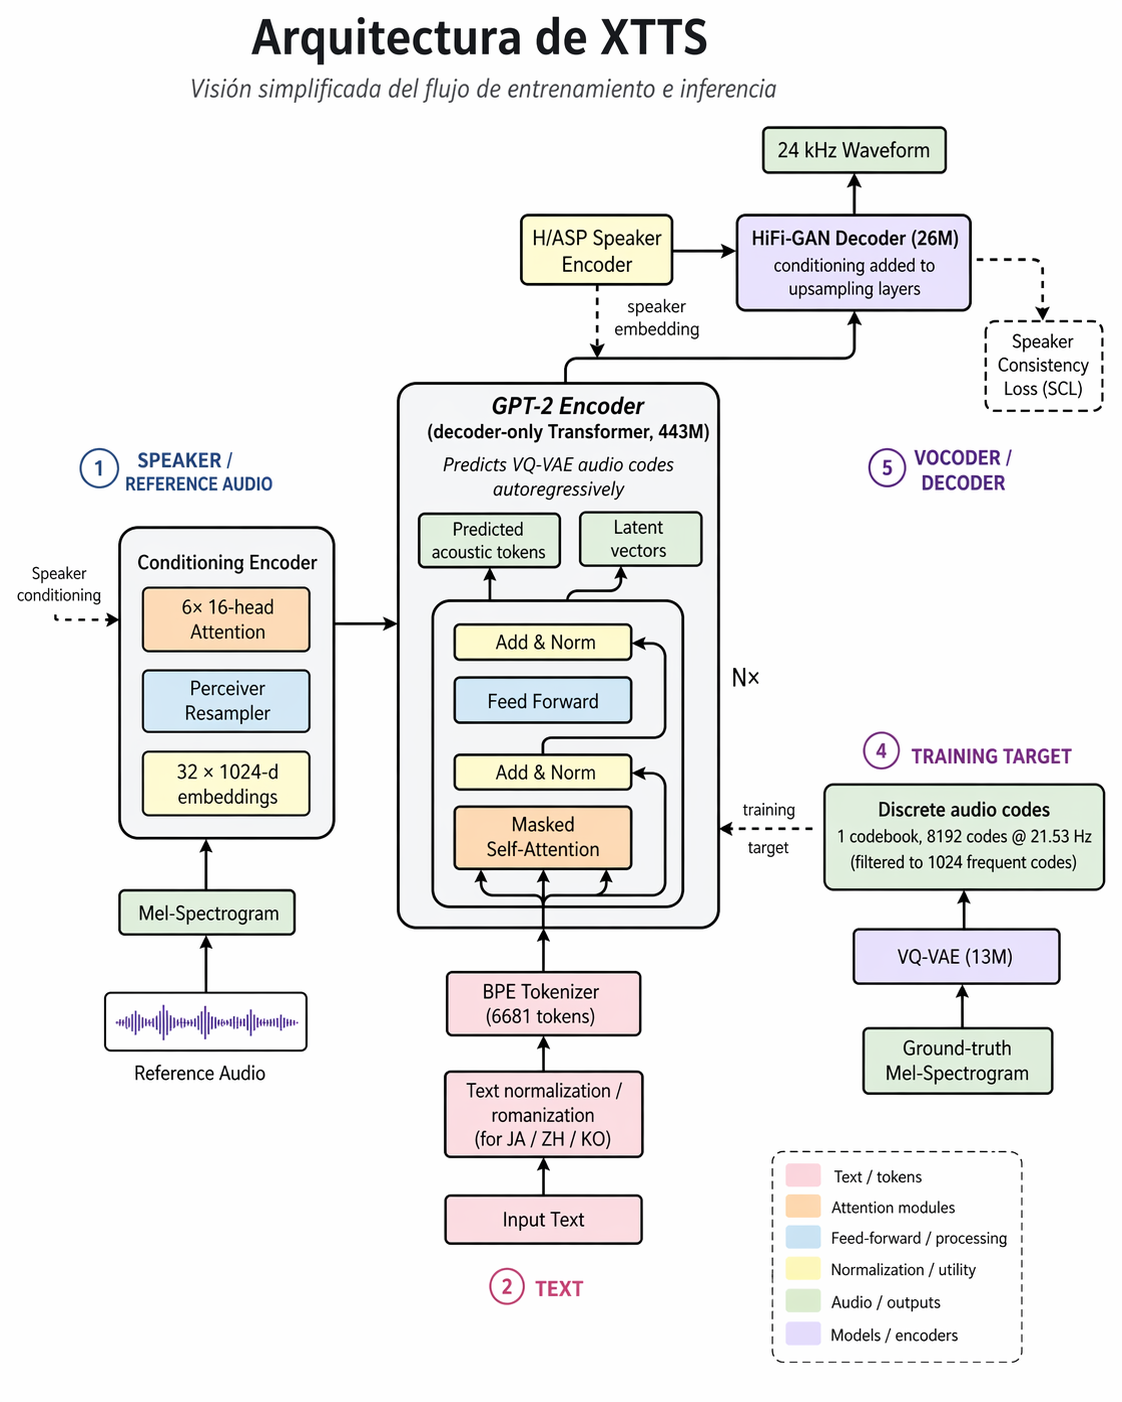
\includegraphics[width=0.9\textwidth]{Imagenes/Propias/Xtts.png}
    \caption[Diagrama general del flujo de XTTS]{
    Diagrama general del flujo de XTTS a partir de texto de entrada y audio de referencia. Fuente: elaboración propia asistida por GPT-Images-2.0 de OpenAI.
    }
    \label{fig:xtts-arquitectura}
\end{figure}

Esta arquitectura permite generar una voz condicionada por una referencia corta de audio, manteniendo cierta identidad del hablante sin necesidad de entrenar un modelo específico desde cero para cada comentarista.

\subsection{Papel de la síntesis de voz dentro del pipeline}

En el contexto de este proyecto, la síntesis de voz transforma los comentarios generados por el modelo de lenguaje en una narración audible. Esta fase cierra el flujo del sistema, convirtiendo eventos detectados y comentarios textuales en audio sincronizable con el vídeo.

En una tarea de narración deportiva, no basta con que la voz generada sea inteligible. También resultan importantes la latencia, la expresividad, la naturalidad en español y la capacidad de mantener un estilo consistente. Por este motivo, el módulo de TTS debe producir audio con suficiente calidad, pero también con un coste temporal asumible dentro del pipeline.

La implementación concreta del módulo de síntesis de voz se describe posteriormente en la \hyperref[sec:sintesis-voz-pipeline]{Sección~\ref*{sec:sintesis-voz-pipeline}}.
